\chapter{Evaluation}

\section{Introduction}

Testing so far has comprised of using small contrived programs to test that statements work individually, and that a few statements work together as they should. However, to test that the designed coverage tools work in the real world, a real piece of software that is written in EOL will be studied. Conveniently Epsilon includes EuGENia which is written in EOL, and also has a test suite, making it the ideal candidate for a case study.

\section{Implementation}

All tests up to this point have been executed by creating an instance of EolParserWorkbench, and then calling functions that parse and execute a test file. However, we now need to execute EuGENia's test suite which is a bit more difficult. To do this, the class EugeniaActionDelegate was modified to include code that adds the execution listeners for statement and branch analysis before execution occurs, but after the EuGENia source has been parsed, so that the AST of the program is available.

The EuGENia source code has two import statements at the top. These import statements were removed, and the files that they referred to were appended to the main source code file. This is because both statement and branch coverage have both been designed with only one source file in mind, which is a shortcoming that will be discussed in the further work section of the conclusion.

\section{Problems}

Statement coverage worked as expected, but branch coverage had two major problems that were spotted after some inspection of the output. 

\subsection{Conditional Branches}

\begin{figure}
\centering
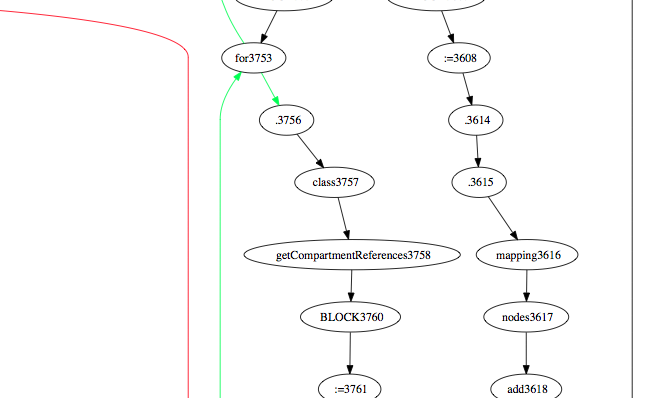
\includegraphics[scale=0.3]{figures/caseStudyProblem1}
\caption{The first problem with branch analysis of EuGENia}
\label{fig:caseStudyProblem1}
\end{figure}

The first problem was that when a conditional statement contained an operation call as part of the condition statement, this executing was causing the branch from the conditional statement to be marked as executed, regardless of whether the block of the conditional statement was actually being executed. An example of this is shown in Figure \ref{fig:caseStudyProblem1}. The for loop header contains the code \verb|class.getCompartmentReferences()| which is split into 3 vertices immediately following the for loop vertex. These are evaluated every time the for loop is reached, and if they return true then the for loop block is executed, and if not the loop is skipped. However, the branch execution listener code was noting that when any of the three vertices were executed that they satisfied the criteria:

\begin{enumerate}
\item The executed vertex is a child of the last executed vertex
\item The CFG of the executed vertex is a child of the CFG of the last executed vertex
\item The executed vertex is a valid type (i.e. whitelisted)
\end{enumerate}

With these conditions satisfied, the branch was being marked as having been executed. Two possible solutions were available. The first is to modify the AST to CFG conversion so that the vertices in the conditional statement are not executed. An attempt was made to implement this solution, but because of how the conversion algorithm deals with the case where there is no code following a loop block, it was not possible to do this `cleanly' (i.e. without lots of nasty conditional statements that would likely introduce bugs). Instead, the branch execution listener was modified so that the extra condition was included:

\begin{enumerate}
\setcounter{enumi}{3}
\item If the parent vertex is of type HELPERMETHOD then this vertex must be of type BLOCK
\end{enumerate}

The additional condition ensures that only the execution of a block under a conditional statement will cause the branch to be marked as executed.

\subsection{Operations}

Simple operation calls were covered during testing, and were thought to work correctly. However, while studying the output of branch analysis on the EuGENia source code, it was apparent that something was not working correctly as some branches were showing that no children had been executed, despite the fact that there definitely should have been at least one child executed (such as at an if .. else statement). An investigation of the cause showed that the problem was limited to when there was an operation call just prior to the problem conditional statement. In the branch execution listener there is a pointer to the last executed vertex that is used when calculating which branch has been executed. When an operation is called, the pointer will be updated within that operation. When control returns to the code that called the operation, the pointer will still be pointing to a vertex within the previously called operation. So when a branch is executed, the branch execution listener will decide that there is no connection between the last executed vertex pointer and the branch that has been executed, and not mark the branch as been executed as it should do.

To solve this problem, a stack was introduced. The idea was that when an operation call is executed the last executed vertex pointer is pushed to the stack, and when the operation call has completed, the stack is popped and stored in the last executed vertex pointer. The implementation was not quite as easy as it could have been. A function had to be implemented that determined whether an operation call had been executed by looking at the relative positions of the last executed vertex and the current executed vertex in the AST. The contents of the stack also have to be checked at each vertex execution because it seems that sometimes the execution listener doesn't always fire the end of an operation call vertex, and it can be necessary to pop more than one pointer from the stack on some occasions. 

\subsection{Path Coverage}

Unfortunately due to time constraints, and also the page limit of this report, I can not fully detail path coverage, and therefore I am counting it as not implemented for the purpose of evaluation and conclusion. In reality much of the work was done for path coverage, and what documentation was made will be included in the appendix.

\section{Results}

\subsection{Statement Coverage}

The results of the statement coverage are found in Appendix \ref{App:StatementCoverage}. The coverage of the existing test suite for EuGENia is 49\%. The output from the analysis clearly shows which section of the code have not been executed, and what needs to be tested in new test suites. For example, the for loop that `Processes EAttributes' (according to the comment above it) is never executed, and so none of the tests must contain models with EAttributes.

A lot of the non-executed statements are those in functions that were originally in the includes, Formatting.eol and ECoreUtil.eol. Despite the criticism of statement coverage that was outlined in the literature review, it is clear that it is sufficient for outlining some major gaps in the EuGENia test suite.

\subsection{Branch Coverage}

Out of 235 branches in EuGENia, 143 were executed (60.9\%). The graph that is produced is very large, too big to include as a whole graph. Instead the output code was modified to print operations as separate graphs so that they can be included more easily in Appendix. It is notable that the percentage of branches that were executed is higher than the percentage of overall statements that were covered. In a review of the statement coverage implementation it was noted that some statements are never marked as being executed, and so the percentage value is of less use that the highlighted syntax output.

% svn diff http://dev.eclipse.org/svnroot/modeling/org.eclipse.epsilon/trunk/plugins/org.eclipse.epsilon.eugenia/transformations/ECore2GMF.eol --revision 100:200 > output2.txt

\subsection{Requirements}

Earlier in the project a set of function and non-functional requirements were detailed. Each of these is now reviewed in Table \ref{tab:Functional}, with a discussion on if and how they have been satisfied.

\begin{table}[h]
    \begin{tabular}{|l|l|p{4.5in}|} \hline
    Requirement & Status        & Justification                                                                                                                                                                                   \\\hline
    F-01        & Satisfied     & It is possible to perform statement coverage on any EOL file with the statement coverage tool that has been implemented.                                                                        \\\hline
    F-02        & Satisfied     & The output HTML file contains the number of statements that have been executed.                                                                                                                 \\\hline
    F-03        & Satisfied     & The output HTML file highlights which statements have been executed, and does not highlight those that have not been executed.                                                                  \\\hline
    F-04        & Satisfied     & It is possible to perform branch coverage on any EOL file with the branch coverage tool that has been implemented.                                                                              \\\hline
    F-05        & Satisfied     & The output from the branch coverage analysis contains a text file that states the number of branches that have been executed.                                                                   \\\hline
    F-06        & Satisfied     & The generated control flow graph highlights branches that have been executed in green, and those that have not are highlighted in red.                                                          \\\hline
    F-07        & Not Satisfied & The user cannot perform path coverage on any EOL file because time limitations prevented this from being completed. However, the majority of the work has been done to implement path coverage. \\\hline
    F-08        & Not Satisfied & Because the user cannot perform path coverage, the number of executed paths cannot be determined.                                                                                               \\\hline
    F-09        & Not Satisfied & Because the user cannot perform path coverage, the user cannot see which paths were executed, and which were not.                                                                               \\\hline
    \end{tabular}
    \caption{Evaluation of functional requirements}
    \label{tab:Functional}
\end{table}

With the non-functional requirements it is a little more difficult to say for sure whether they have been satisfied or not. There were two core requirements, repeated for each of the three coverage types. The first core requirement was that the coverage analysis will not take an `excessive' amount of time to complete. What is excessive can only be decided by the user. In my experience, the tools that were investigated during the literature review did not add more than 5 seconds to the overall execution time of a test suite.

%Baseline: 56.9, 52.4, 53.6
%Statement: 62.9, 63.2, 62.3
%Branch: 68.4, 65.9, 65.7

The execution time of the EuGENia test suite was recorded with no coverage analysis enabled, with statement coverage enabled, and finally with branch coverage enabled. Each test was run three times, with the average and standard deviation recorded. The results are shown in Table \ref{tab:runTimes}.

\begin{table}[h]
\centering
    \begin{tabular}{|p{1in} | p{0.6in} |p{0.6in} |p{0.6in} |p{0.6in} |p{0.8in} |} \hline
    Coverage Type & Time 1 (seconds) & Time 2 (seconds) & Time 3 (seconds) & Average Time (seconds) & Standard Deviation (seconds) \\\hline
    None          & 56.9             & 52.4             & 53.6             & 54.3                   & 2.3                          \\\hline
    Statement     & 62.9             & 63.2             & 62.3             & 62.8                   & 0.5                          \\\hline
    Branch        & 68.4             & 65.9             & 65.7             & 66.7                   & 1.5                          \\\hline
    \end{tabular}
    \caption{Run Times of the EuGENia test suite}
    \label{tab:runTimes}
\end{table}

It is interesting to note that both statement and branch coverage increase the run time quite significantly (15\% and 23\%, respectively). A more careful analysis showed that the slowdown was not in the analysis and output of the statistics, but in the execution listener code. I find it to be surprising that the statement coverage code slows the execution down by such a lot, because the execution listener really does not do a great deal.

On the other hand, the speed of the branch analysis does not come as a surprise. As each statement is executed, a partial traversal of the AST is performed to determine if the executed statement is in the same operation as the previously executed statement, and this will cause a slowdown.

While it is purely subjective, I am going to say that the core requirements for statement and branch coverage have been satisfied. I will discuss possible further work to speed up the code in the next chapter. Because path coverage has not been completely implemented, I am counting the related core non-functional requirements as not satisfied.